%
% $RCSfile: data_mapper.tex,v $
%
% Copyright (c) 2001-2004. Christian Heller. All rights reserved.
%
% No copying, altering, distribution or any other actions concerning this
% document, except after explicit permission by the author!
% At some later point in time, this document is planned to be put under
% the GNU FDL license. For now, _everything_ is _restricted_ by the author.
%
% http://www.cybop.net
% - Cybernetics Oriented Programming -
%
% http://www.resmedicinae.org
% - Information in Medicine -
%
% @author Christian Heller <christian.heller@tuxtax.de>
%

\subsection{Data Mapper}
\label{data_mapper_heading}

Originally, the communication approach of CYBOP was based on the
\emph{Data Mapper} pattern (figure \ref{data_mapper_figure}).
\begin{figure}[ht]
    \begin{center}
       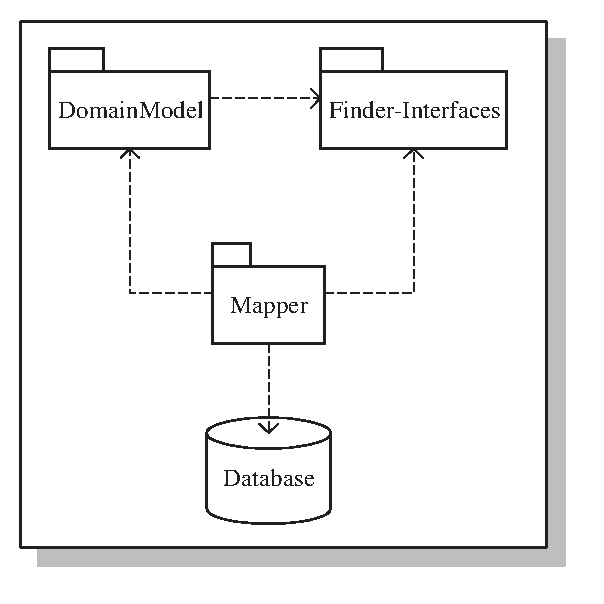
\includegraphics[scale=0.6]{vector/data_mapper.eps}
       \caption{Data Mapper Design Pattern \cite{fowler2002}}
       \label{data_mapper_figure}
    \end{center}
\end{figure}

It is part of Martin Fowler's pattern collection called \emph{Enterprise Application
Architecture} \cite{fowler2002}. The most important idea of this pattern is to
abolish the interdependency of domain (knowledge) model and database (persistence).\\
The arrows in figure \ref{data_mapper_figure} indicate the direction of dependency.
Each domain model class knows its appropriate persistence finder interface but
does not know their implementation, i.e. how data are actually retrieved from
the database. The data mapper implementation is part of the mapping package that
implements all finders and maps all data of the received result set to the special
attributes of the domain model objects.
There is no need for the domain model to know where the database is located or
how to get the data -- and also not how to map the entity-relationship model data.\\
If all these things are done by the corresponding data mappers now, why shouldn't
it be possible to get such a mapping package for persistence media of any kind,
no matter which communication paradigm (File Stream, JDBC with SQL) is used?
Users would have a number of persistence mechanisms to dynamically choose from;
developers would not have to implement the same mechanisms again and again for
each new module (application) -- leading to clearer code with greatly reduced size.\\
This functional code separation would make it easy to develop a complicated
domain model and update it later, if necessary. The data mapper package could
contain special parts for local storage in a file system, in various file formats
such as XML, CSV, TXT etc. (whether it makes sense or not to store domain data
in a pure text file), for a number of (relational) databases (PostgreSQL, MySQL)
and so on.
Each of those specialised parts would know how to communicate with its appropriate
persistence medium and only with it. They would all include a specialised mapper
class, called \emph{Translator} in CYBOP, which translates the data from the
domain model to the model of the corresponding persistence mechanism.

